% GBA Fuse & Cable Protection Tool — Engineering Brief
% GB Engineering · Version 2 · GBA-0002
\documentclass[11pt,a4paper]{report}

\usepackage[utf8]{inputenc}
\usepackage[T1]{fontenc}
\usepackage[margin=25mm]{geometry}
\usepackage{amsmath,amssymb}
\usepackage{booktabs}
\usepackage{longtable}
\usepackage{array}
\usepackage{hyperref}
\usepackage{graphicx}
\usepackage{enumitem}
\usepackage{xcolor}
\usepackage{listings}
\usepackage{tikz}
\usetikzlibrary{shapes.geometric, arrows.meta, positioning, fit}

\hypersetup{
  colorlinks=true,
  linkcolor=blue!60!black,
  citecolor=blue!60!black,
  urlcolor=blue!60!black,
  pdftitle={GBA Fuse Tool Engineering Brief},
  pdfauthor={GB Engineering}
}

\lstdefinestyle{ts}{
  language=Java,
  basicstyle=\ttfamily\small,
  keywordstyle=\color{blue},
  commentstyle=\color{gray},
  stringstyle=\color{teal},
  breaklines=true,
  frame=single,
  rulecolor=\color{black!20},
  tabsize=2
}

\title{%
  \textbf{GB Auto Fuse \& Cable Protection Tool}\\[0.4em]
  \large Engineering Brief for Electrical and Software Teams\\[0.2em]
  \normalsize Document GBA-0002 · Version 2
}
\author{GB Engineering}
\date{June 2026}

\begin{document}
\maketitle

\begin{abstract}
This document briefs electrical, software, and multidisciplinary engineers on the GB Auto Fuse and Cable Protection web application. It presents the electrical theory and equations implemented in the calculation engine, the software architecture and code logic, traceability to specification GBA-0002, known limitations, and guidance for client-facing communication. The tool replaces a legacy Excel workbook and incomplete MATLAB prototype with a tested TypeScript engine, normalized JSON data libraries, and a mobile-friendly Next.js user interface.
\end{abstract}

\tableofcontents
\newpage

%=============================================================================
\chapter{Introduction and scope}
%=============================================================================

\section{Purpose of the tool}

Heavy machinery on mine sites and civil fleets typically operates on \textbf{24\,V} starting circuits. During engine cranking, the starter motor draws hundreds to thousands of amperes for several seconds. The battery, starter cable, and fuse must be coordinated so that:

\begin{itemize}[noitemsep]
  \item the cable carries \textbf{continuous} alternator current after start;
  \item the cable survives \textbf{short-time cranking} current without thermal damage;
  \item voltage drop at the starter remains acceptable;
  \item the fuse is sized above normal load but withstands cranking without nuisance blowing;
  \item the fuse \textbf{protects} the cable from sustained overcurrent.
\end{itemize}

The web application automates these checks using fleet data and manufacturer libraries (cable capacity, Littelfuse MEGA\,32\,V fuses, copper adiabatic constants). Outputs are \textbf{decision-support recommendations}---not certified design sign-off.

\section{Document audience}

\begin{table}[h]
  \centering
  \caption{Intended readers and focus areas}
  \begin{tabular}{@{}ll@{}}
    \toprule
    \textbf{Role} & \textbf{Use this document to\ldots} \\
    \midrule
    Electrical engineer & Verify equations, assumptions, gaps vs.\ standards \\
    Software engineer & Understand module boundaries, APIs, tests \\
    Project / client lead & Prepare accurate client responses (Chapter~\ref{ch:client}) \\
    Other engineers & Gain circuit context without reading source code \\
    \bottomrule
  \end{tabular}
\end{table}

\section{Version history}

\begin{itemize}[noitemsep]
  \item \textbf{Phase 1 (\texttt{main}):} Library mode, core cable/fuse checks, Excel data migration.
  \item \textbf{Engineering V2 (\texttt{main}):} Completeness gate, manual entry, full check cards, fuse-protects-cable.
  \item \textbf{Client v0 (\texttt{client/v0}):} Minimal GBA-0002 prototype --- four user inputs, nine sample machines, \texttt{gba0002/} engine only in UI.
  \item \textbf{Client v1 (\texttt{client/v1}):} Full GBA-0002 trace UI and client deliverable documentation.
  \item \textbf{Client v2 (\texttt{client/v2}):} Client v1 plus layered input/output validation guardrails.
  \item \textbf{Planned:} Parallel fuses, admin UI, PDF export, installation derating.
\end{itemize}

\section{Repository layout}

\begin{verbatim}
fuse-tool/
  apps/web/           Next.js 15 + Tailwind UI (client)
  packages/engine/    @fuse-tool/engine pure TypeScript (calculations)
  data/               JSON libraries exported from Fuse_GUI_APP.xlsx
  scripts/            import_from_xlsx.py
  docs/               Specifications, user guide, this brief
\end{verbatim}

%=============================================================================
\chapter{Electrical theory and circuit context}
%=============================================================================

\section{Single-line model}

The analysed circuit is simplified to:

\[
  \text{Battery} \rightarrow \text{Fuse} \rightarrow \text{Cable (out \& return)} \rightarrow \text{Starter motor}
\]

During cranking, current is dominated by starter torque demand. After start, current falls to alternator charging and vehicle loads. The fuse must protect the cable under fault and overload while not opening during legitimate cranking.

\section{Typical 24\,V boundary conditions}

Values align with project documentation and \texttt{data/constants.json}:

\begin{table}[h]
  \centering
  \caption{Electrical boundary conditions (typical)}
  \begin{tabular}{@{}lll@{}}
    \toprule
    \textbf{Parameter} & \textbf{Typical value} & \textbf{Source} \\
    \midrule
    System voltage $V_\mathrm{sys}$ & 24\,V & Machine record or manual entry \\
    Minimum battery voltage $V_\mathrm{min}$ & 16.48\,V & Constants (16\,V + 3\%) \\
    Peak cranking limit $I_\mathrm{limit}$ & 500--1000\,A & Per machine \texttt{peakCurrentCutoffA} \\
    Cranking current $I_\mathrm{crank}$ & 200--1000\,A & Measured / specified \\
    Cranking time $t$ & $\geq 5$\,s floor & \texttt{max}(t_\mathrm{meas}, 5\,\mathrm{s}) \\
    Alternator continuous $I_\mathrm{alt}$ & 80--150\,A & Machine / manual entry \\
    Voltage drop limit & 3\% & Configurable constant \\
    Fuse safety factor & 25\% & Configurable (default) \\
    \bottomrule
  \end{tabular}
\end{table}

\section{Applicable standards (reference)}

The tool references (but does not automatically enforce full compliance with):

\begin{itemize}[noitemsep]
  \item AS/NZS\,5000.1 --- electric cables, extruded insulation;
  \item AS/NZS\,1125 --- conductors in electric cables;
  \item AS/NZS\,1995:2003 --- welding cable duty cycles (reference for cranking duty).
\end{itemize}

IEC and SAE references appear in the broader project plan for future library expansion. \textbf{Engineers must confirm} installation method, grouping, ambient temperature, and OEM requirements beyond what Version~2 calculates.

%=============================================================================
\chapter{Equations and calculation rules}
%=============================================================================

All equations below are implemented in \texttt{@fuse-tool/engine}. Each produces a \texttt{CheckResult} with status \texttt{pass}, \texttt{fail}, \texttt{warning}, \texttt{unavailable}, or \texttt{invalid}.

\section{Battery checks}

\subsection{Cranking voltage}

Compare measured voltage during cranking to minimum allowable battery voltage:
\begin{equation}
  \text{Pass if } V_\mathrm{crank} \geq V_\mathrm{min}
\end{equation}
Implemented only when both values are present (library data or manual optional fields). A fail flags battery investigation or replacement.

\subsection{Cranking time}

Compare measured cranking duration to allowed maximum:
\begin{equation}
  \text{Pass if } t_\mathrm{meas} \leq t_\mathrm{allowed}
\end{equation}

\section{Starter motor cranking current}

The engine does \textbf{not} calculate cranking current from mechanical power in Version~2. It uses stored or manually entered $I_\mathrm{crank}$ and compares to the machine peak limit:
\begin{equation}
  \text{Pass if } I_\mathrm{crank} \leq I_\mathrm{limit}
\end{equation}
where $I_\mathrm{limit}$ is \texttt{peakCurrentCutoffA} per vehicle, or \texttt{defaultPeakCrankingLimitA} from constants when absent.

\textbf{GBA-0002 note:} The specification describes deriving cranking current from starter motor electrical power:
\begin{equation}
  I_\mathrm{crank} = \frac{P_\mathrm{elec}}{V_\mathrm{starter}}
  = \frac{P_\mathrm{mech}/\eta}{V_\mathrm{starter}}
\end{equation}
Starter motor library data is imported into machine records but lookup-based calculation is deferred to a future release.

\section{Cable continuous-current check}

The alternator continuous output must not exceed the cable's rated continuous current:
\begin{equation}
  \text{Pass if } I_\mathrm{alt} \leq I_\mathrm{cable,cont}
\end{equation}
\textbf{Version~2 limitation:} No installation derating (ambient, grouping, enclosure) is applied. Ratings are taken as entered or from the fleet record.

\section{Cable inrush / adiabatic peak capability}

For short-duration cranking, copper conductors may carry current above continuous rating using the \textbf{adiabatic equation}:
\begin{equation}
  I_\mathrm{allow} = \frac{K \cdot S}{\sqrt{t}}
  \label{eq:adiabatic}
\end{equation}
where:
\begin{itemize}[noitemsep]
  \item $K$ = copper constant (A$\cdot\sqrt{\mathrm{s}}$/mm$^2$) from \texttt{Copper\_K\_Factor} (column~A) matched by \textbf{cable type} from MachinesOnSite column~AD --- not by machine model;
  \item $S$ = conductor cross-section (mm$^2$);
  \item $t$ = cranking time used for the check (seconds).
\end{itemize}

\textbf{Pass rule:}
\begin{equation}
  I_\mathrm{crank} \leq I_\mathrm{allow}
\end{equation}

\textbf{Required cranking time:}
\begin{equation}
  t_\mathrm{req} = \max(t_\mathrm{meas}, t_\mathrm{min}), \quad t_\mathrm{min} = 5\,\mathrm{s}
\end{equation}

\textbf{Validity window:} If $t > \texttt{maxAdiabaticCrankingTimeS}$ (5\,s), the engine returns \texttt{warning}---the adiabatic model is not intended for extended cranking; investigate mechanical or battery faults.

\textbf{Legacy correction:} The Excel workbook erroneously used $t = 15/1000$\,s in $\sqrt{t}$ (cell G13). The engine uses actual cranking time.

\textbf{Inverse (maximum time for given current):}
\begin{equation}
  t_\mathrm{max} = \left(\frac{K \cdot S}{I_\mathrm{crank}}\right)^2
\end{equation}

\subsection{Typical $K$ values (copper)}

\begin{table}[h]
  \centering
  \begin{tabular}{@{}lc@{}}
    \toprule
    Insulation / type & $K$ (approx.) \\
    \midrule
    Thermoplastic 70\,°C PVC & 115 \\
    Thermoplastic 90\,°C PVC & 100 \\
    Thermosetting 90\,°C XLPE & 143 \\
    Thermosetting 60\,°C rubber & 141 \\
    \bottomrule
  \end{tabular}
\end{table}

\section{Voltage drop}

Round-trip resistance (out and return conductors):
\begin{equation}
  R_\mathrm{total} = 2 \cdot L \cdot \frac{R_{\Omega/\mathrm{km}}}{1000}
\end{equation}
Voltage drop and percentage:
\begin{equation}
  \Delta V = I_\mathrm{crank} \cdot R_\mathrm{total}, \qquad
  \Delta V\% = \frac{\Delta V}{V_\mathrm{base}} \times 100
\end{equation}
$R_{\Omega/\mathrm{km}}$ is looked up from \texttt{cable-capacity.json} by cable size. $V_\mathrm{base}$ is system voltage or measured cranking voltage when available.

\textbf{Pass/warning:} $\Delta V\% \leq$ voltage drop limit (default 3\%). Exceeding the limit yields \texttt{warning} in the full engineering tool (\texttt{main}).

\subsection{Client GBA-0002 voltage budget (absolute volts)}

The simplified client application (branches \texttt{client/v0}--\texttt{client/v2}) uses the user-entered \textbf{battery voltage during cranking} and a fixed minimum starter voltage of \textbf{16\,V}:
\begin{equation}
  \Delta V_\mathrm{max} = V_\mathrm{battery,cranking} - 16\,\mathrm{V}
\end{equation}
This is the voltage \emph{budget} available for cable loss (out and return) while maintaining at least 16\,V at the starter terminals. It is not a percentage drop. See \texttt{docs/GBA0002\_ENGINEERING\_THEORY.md} for the engineering rationale.

Maximum one-way cable length from this budget:
\begin{equation}
  L_\mathrm{max} = \frac{\Delta V_\mathrm{max} \times 1000}{I_\mathrm{crank} \times 2 \times R_{\Omega/\mathrm{km}}}
\end{equation}
Implemented in \texttt{packages/engine/src/gba0002/calculate.ts}.

\section{I\textsuperscript{2}t thermal energy}

Thermal energy associated with a current pulse:
\begin{equation}
  \mathrm{I}^2 t = I^2 \cdot t \quad [\mathrm{A}^2\mathrm{s}]
\end{equation}
\textbf{Example:} $1000\,\mathrm{A}$ for $5\,\mathrm{s}$ $\Rightarrow$ $5 \times 10^6\,\mathrm{A}^2\mathrm{s}$.

Fuse withstand time from I\textsuperscript{2}t rating (supplementary):
\begin{equation}
  t_\mathrm{fuse} = \frac{(\mathrm{I}^2 t)_\mathrm{fuse}}{I^2}
\end{equation}

The engine uses I\textsuperscript{2}t as a \textbf{supplementary audit check}. Primary fuse cranking validation uses the MEGA\,32\,V time-current graph.

\section{Fuse continuous rating (safety factor)}

When the cable continuous check passes:
\begin{equation}
  I_\mathrm{fuse,target} = \left(1 + \frac{s}{100}\right) \cdot I_\mathrm{alt}
\end{equation}
Default safety factor $s = 25\%$ $\Rightarrow$ multiply by $1.25$.

\textbf{Example:} $I_\mathrm{alt} = 389\,\mathrm{A}$, $s=25\%$ $\Rightarrow$ $I_\mathrm{fuse,target} = 486.25\,\mathrm{A}$.

\section{Fuse library selection}

The closest standard rating from \texttt{fuse-library.json} minimizes $|I_\mathrm{rating} - I_\mathrm{fuse,target}|$.

\section{Fuse time-current withstand (MEGA\,32\,V)}

For breaking current $I_\mathrm{break}$ (typically peak cranking limit) and selected fuse rating, the engine looks up withstand time $t_\mathrm{withstand}$ from \texttt{mega32v-curve.json} or fuse record \texttt{timeFromGraphS}.

\textbf{Pass rule:}
\begin{equation}
  t_\mathrm{withstand} \geq t_\mathrm{req}
\end{equation}

If insufficient, the engine \textbf{escalates} to the next standard fuse rating (up to 8 steps) and re-evaluates.

\section{Fuse protects cable}

The selected fuse must not exceed cable continuous rating (derating not applied in V2):
\begin{equation}
  \text{Pass if } I_\mathrm{fuse,selected} \leq I_\mathrm{cable,cont}
\end{equation}

\section{Parallel fuses (not implemented)}

GBA-0002 defines:
\begin{align}
  I_\mathrm{per\,fuse} &= \frac{I_\mathrm{total}}{n} \\
  I_\mathrm{derated} &= I_\mathrm{fuse} \cdot n \cdot f_\mathrm{parallel}
\end{align}
Parallel fuse logic (Excel G55--G57) is planned for Version~3.

\section{Overall result aggregation}

Each check returns a status. The summary uses the \textbf{worst} status in priority order:
\[
  \texttt{fail} > \texttt{invalid} > \texttt{warning} > \texttt{unavailable} > \texttt{pass}
\]
Cable and fuse \textbf{suitability badges} on the GBA-0002 output panel aggregate subsets of checks (see \texttt{outputs.ts}).

%=============================================================================
\chapter{Data libraries and traceability}
%=============================================================================

\section{JSON data sources}

\begin{longtable}{@{}p{3.2cm}p{4.5cm}p{6cm}@{}}
  \toprule
  \textbf{File} & \textbf{Excel sheet} & \textbf{Content} \\
  \midrule
  \endhead
  \texttt{machines.json} & MachinesOnSite & Fleet vehicles, cranking data, cable fields \\
  \texttt{cable-capacity.json} & Cable\_Capacity & Size, continuous $I$, $R_{\Omega/\mathrm{km}}$ \\
  \texttt{fuse-library.json} & Fuse\_Library & Ratings, I\textsuperscript{2}t, part numbers \\
  \texttt{mega32v-curve.json} & MEGA32V & Time-current withstand matrix \\
  \texttt{copper-k-factors.json} & Copper\_K\_Factor & Adiabatic $K$ by insulation \\
  \texttt{constants.json} & User Input / MD6250 & Defaults, standards list \\
  \bottomrule
\end{longtable}

Regenerate from Excel: \texttt{npm run import:data} (\texttt{scripts/import\_from\_xlsx.py}).

\section{Vehicle completeness (Version 2)}

Full recommendations require all fields in \texttt{REQUIRED\_FIELDS} (\texttt{completeness.ts}):

\begin{itemize}[noitemsep]
  \item \texttt{peakCrankingCurrentA}, \texttt{alternatorContinuousA}
  \item \texttt{cableType}, \texttt{cableSizeMm2}, \texttt{cableContinuousA}, \texttt{cableLengthM}, \texttt{operatingTempC}
  \item \texttt{peakCurrentCutoffA}, \texttt{electricalSystemV}
  \item Cranking time (measured or required)
\end{itemize}

As of Version~2, \textbf{9 of 37} fleet records are complete. Incomplete records remain visible but \texttt{blocked: true} prevents partial unsafe outputs.

%=============================================================================
\chapter{Software architecture}
%=============================================================================

\section{Design principles}

\begin{enumerate}[noitemsep]
  \item \textbf{Separation of concerns:} All calculations live in \texttt{@fuse-tool/engine}; the web UI only renders results.
  \item \textbf{Pure functions:} Cable and fuse modules are deterministic given inputs and database snapshots.
  \item \textbf{Auditable outputs:} Every check includes \texttt{specification}, \texttt{message}, and optional \texttt{legacyReference}.
  \item \textbf{Fail-safe data handling:} Incomplete library vehicles and invalid manual input are blocked before calculation.
  \item \textbf{Configuration over hard-coding:} Defaults load from \texttt{constants.json}; assumptions listed in \texttt{derived.assumptionsUsed}.
  \item \textbf{Test-driven regression:} Vitest golden vectors (e.g.\ B45E) and Version~2 acceptance tests.
\end{enumerate}

\section{Technology stack}

\begin{table}[h]
  \centering
  \begin{tabular}{@{}ll@{}}
    \toprule
    Layer & Technology \\
    \midrule
    UI & Next.js 15, React, Tailwind CSS \\
    Engine & TypeScript (ES modules), compiled with \texttt{tsc} \\
    Tests & Vitest \\
    Data & JSON (imported from Excel) \\
    Deployment & Vercel / Netlify (static + SSR) \\
    \bottomrule
  \end{tabular}
\end{table}

\section{Calculation pipeline}

\begin{figure}[h]
  \centering
  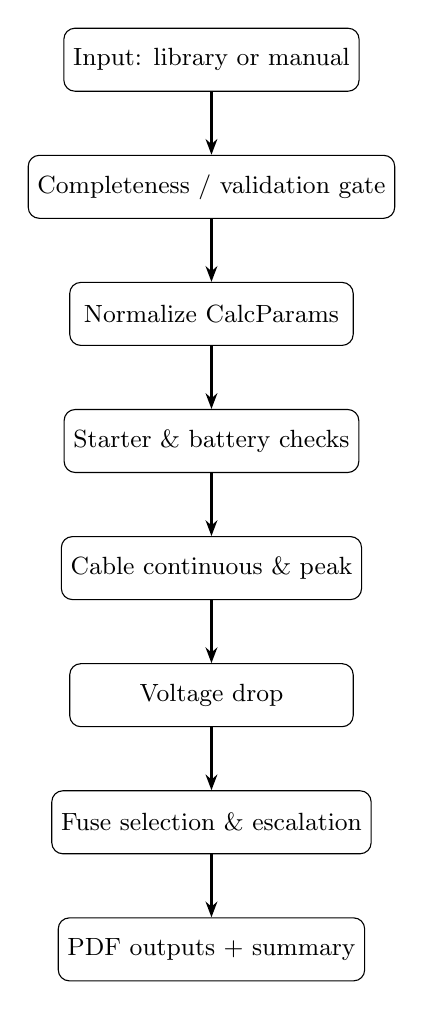
\begin{tikzpicture}[
    node distance=8mm,
    box/.style={draw, rounded corners, minimum width=3.6cm, minimum height=8mm, align=center, font=\small},
    arr/.style={-{Stealth[length=2mm]}, thick}
  ]
    \node[box] (in) {Input: library or manual};
    \node[box, below=of in] (gate) {Completeness / validation gate};
    \node[box, below=of gate] (params) {Normalize CalcParams};
    \node[box, below=of params] (starter) {Starter \& battery checks};
    \node[box, below=of starter] (cable) {Cable continuous \& peak};
    \node[box, below=of cable] (vdrop) {Voltage drop};
    \node[box, below=of vdrop] (fuse) {Fuse selection \& escalation};
    \node[box, below=of fuse] (out) {PDF outputs + summary};
    \draw[arr] (in) -- (gate);
    \draw[arr] (gate) -- (params);
    \draw[arr] (params) -- (starter);
    \draw[arr] (starter) -- (cable);
    \draw[arr] (cable) -- (vdrop);
    \draw[arr] (vdrop) -- (fuse);
    \draw[arr] (fuse) -- (out);
  \end{tikzpicture}
  \caption{High-level calculation flow (\texttt{calculate.ts})}
\end{figure}

\section{Module reference}

\begin{longtable}{@{}p{3.5cm}p{9.5cm}@{}}
  \toprule
  \textbf{Module} & \textbf{Responsibility} \\
  \midrule
  \endhead
  \texttt{calculate.ts} & Orchestrator: gates, \texttt{runFullCalculation}, \texttt{recommend()} wrapper \\
  \texttt{cableChecks.ts} & Continuous and adiabatic peak; voltage drop formula \\
  \texttt{fuseSelection.ts} & Target rating, closest match, MEGA32V escalation, I\textsuperscript{2}t, protects-cable \\
  \texttt{lookups.ts} & Machine find, $K$-factor, resistance, fuse graph lookup \\
  \texttt{completeness.ts} & Required field assessment for library vehicles \\
  \texttt{validation.ts} & Manual entry field validation \\
  \texttt{outputs.ts} & GBA-0002 cable/fuse output block and suitability aggregation \\
  \texttt{parseValue.ts} & Legacy Excel cell parsing (\texttt{\#VALUE!}, etc.) \\
  \texttt{types.ts} & Shared interfaces: \texttt{CheckResult}, \texttt{RecommendationResult} \\
  \texttt{catalog.ts} & \texttt{loadDatabase}, \texttt{listModelIds} \\
  \texttt{gba0002/calculate.ts} & Client GBA-0002: thermal $(kS/I)^2$, voltage budget, fuse selection \\
  \texttt{gba0002/helpers.ts} & Strict $K$-factor by cable type; temperature range parsing \\
  \texttt{recommendLegacyNotes.ts} & Documented fixes vs Excel/MATLAB \\
  \bottomrule
\end{longtable}

\section{Public API}

Entry point \texttt{calculate(db, request)}:

\begin{lstlisting}[style=ts]
// Library mode
calculate(db, { mode: "library", modelId: "B45E",
  safetyFactorPercent?: number, voltageDropLimitPercent?: number });

// Manual mode
calculate(db, { mode: "manual", inputs: ManualEntryInput });
\end{lstlisting}

Legacy wrapper: \texttt{recommend(db, \{ modelId \})} $\rightarrow$ library mode only.

\textbf{Key result fields:}
\begin{itemize}[noitemsep]
  \item \texttt{blocked} --- true if incomplete or invalid input
  \item \texttt{checks[]} --- auditable check cards
  \item \texttt{fuse} --- target/selected rating, part record, I\textsuperscript{2}t
  \item \texttt{outputs} --- GBA-0002 cable/fuse panel (null when blocked)
  \item \texttt{derived.assumptionsUsed[]} --- transparency for engineers
  \item \texttt{implementationNotes[]} --- legacy bug fixes applied
\end{itemize}

\section{Web application structure}

\textbf{Full engineering tool (\texttt{main}):}
\begin{itemize}[noitemsep]
  \item \texttt{Calculator.tsx} --- library and manual entry modes
  \item \texttt{ManualEntryForm.tsx}, \texttt{CheckCard.tsx}, \texttt{PdfResultsPanel.tsx}
  \item \texttt{lib/db.ts} --- loads \texttt{bundle.json}
\end{itemize}

\textbf{Client GBA-0002 deliverable (\texttt{client/v0}--\texttt{client/v2}):}
\begin{itemize}[noitemsep]
  \item \texttt{Gba0002Calculator.tsx} --- four inputs (safety factor, machine, battery $V$, temperature), Calculate button, results table
  \item \texttt{packages/engine/src/gba0002/} --- \texttt{calculate.ts}, \texttt{helpers.ts} (strict $K$-factor lookup, temperature parsing)
  \item v0: minimal UI and docs only; v1: calculation trace; v2: validation guardrails
\end{itemize}

The UI never implements formulas; it only displays engine output. This allows CLI testing, future mobile apps, and API deployment without duplicating logic.

\section{Testing strategy}

\begin{table}[h]
  \centering
  \caption{Test coverage (\texttt{npm test} --- 26 tests)}
  \begin{tabular}{@{}ll@{}}
    \toprule
    Suite & Coverage \\
    \midrule
    \texttt{recommend.test.ts} & Golden vectors B45E, D10T, high cranking, unknown model \\
    \texttt{v2.test.ts} & Completeness, manual validation, blocked vehicles, fuse-protects-cable \\
    \bottomrule
  \end{tabular}
\end{table}

Tests load real JSON from \texttt{data/} --- no mocked cable/fuse tables --- ensuring import integrity.

\section{Legacy corrections applied}

\begin{table}[h]
  \centering
  \small
  \begin{tabular}{@{}p{1.2cm}p{4cm}p{7cm}@{}}
    \toprule
    ID & Issue & Engine fix \\
    \midrule
    EX-01 & G13 used 0.015\,s in $\sqrt{t}$ & Use cranking time \\
    EX-02 & G31 compared cutoff to capability & Compare $I_\mathrm{crank}$ to $I_\mathrm{allow}$ \\
    EX-03 & G19 compared strings to voltage & Compare $V_\mathrm{crank}$ to $V_\mathrm{min}$ \\
    ML-01 & MATLAB truncated columns A:X & Full machine JSON \\
    ML-03 & Hard-coded $K=143$ & Lookup by cable type (AD$\rightarrow$Copper\_K\_Factor); client branches block if missing \\
    \bottomrule
  \end{tabular}
\end{table}

Full register: \texttt{docs/LEGACY\_BUGS\_FIXED.md}.

%=============================================================================
\chapter{GBA-0002 compliance matrix}
%=============================================================================

\begin{longtable}{@{}p{5.2cm}ccp{4cm}@{}}
  \toprule
  \textbf{Requirement} & \textbf{Main / Client} & \textbf{Planned} & \textbf{Notes} \\
  \midrule
  \endhead
  Machine library selection & \checkmark & & Main: 37 vehicles; client: 9 sample \\
  Manual entry mode & \checkmark & & Main only \\
  Client four-input GBA-0002 UI & \checkmark & & \texttt{client/v0}--\texttt{v2} \\
  Voltage drop (\% limit) & \checkmark & & Main \\
  Voltage budget ($V_\mathrm{bat}-16$\,V) & \checkmark & & Client GBA-0002 \\
  $K$-factor by cable type (strict) & \checkmark & & Client; main uses lookup + fallbacks \\
  Battery voltage / time checks & \checkmark & & When data present \\
  Starter cranking limit & \checkmark & & \\
  Cable continuous \& inrush & \checkmark & & No derating \\
  Voltage drop & \checkmark & & \\
  I\textsuperscript{2}t & \checkmark & & Supplementary \\
  Fuse sizing + library match & \checkmark & & \\
  MEGA32V withstand + escalation & \checkmark & & \\
  Fuse protects cable & \checkmark & & Raw ratings only \\
  GBA-0002 output fields (8 items) & \checkmark & & \\
  Incomplete vehicle blocking & \checkmark & & \\
  Starter motor power $\rightarrow I_\mathrm{crank}$ & & $\circ$ & Uses measured $I$ \\
  Parallel fuse logic & & $\circ$ & \\
  Cable/fuse temperature derating & & $\circ$ & \\
  Fault interrupting rating check & & $\circ$ & \\
  PDF export & & $\circ$ & On-screen only \\
  Admin fleet editor & & $\circ$ & JSON/Excel today \\
  \bottomrule
\end{longtable}

Legend: \checkmark\,implemented; $\circ$\,planned.

%=============================================================================
\chapter{Client communication guide}
\label{ch:client}
%=============================================================================

This chapter helps engineers respond accurately to the client (GB Auto / fleet operator) regarding scope, capability, limitations, and deliverables. Use factual language; avoid over-promising certification or standards compliance the tool does not perform automatically.

\section{Executive summary (client-ready)}

\begin{quote}
\small
We have delivered the Fuse and Cable Protection web application per specification GBA-0002 in several branches: a \textbf{minimal client prototype} (\texttt{client/v0}), a \textbf{client deliverable with full calculation trace} (\texttt{client/v1}), and a \textbf{validated client build} with input guardrails (\texttt{client/v2}), alongside the full \textbf{engineering tool} on \texttt{main} (37-vehicle library, manual entry, completeness gate). All analyse 24\,V starting circuits using fleet data and manufacturer libraries. Outputs are design aids; final selections require qualified engineering review.
\end{quote}

\section{What we delivered}

\begin{enumerate}
  \item \textbf{Web application} --- vehicle library and manual entry modes.
  \item \textbf{Calculation engine} --- documented equations, auditable check cards, legacy Excel/MATLAB corrections.
  \item \textbf{Data migration} --- Excel workbook exported to version-controlled JSON.
  \item \textbf{Documentation} --- user guide, calculation spec, this engineering brief.
  \item \textbf{Automated tests} --- regression protection for fleet golden cases.
\end{enumerate}

\section{What to tell the client about data quality}

\begin{quote}
\small
The fleet library contains 37 machines. \textbf{Nine} currently have complete engineering data for automated full recommendations. The remainder are visible in the list but clearly marked as incomplete; the application lists missing fields and does not produce partial fuse/cable recommendations that could be misinterpreted. Incomplete cases can be analysed via \textbf{Manual entry} once site measurements are available, or fleet records can be updated in the master spreadsheet and re-imported.
\end{quote}

\section{Frequently asked client questions}

\subsection{``Does this replace our Excel tool?''}

\textbf{Response:} For the core starting-circuit checks (cable continuous/peak, voltage drop, fuse sizing, MEGA32V withstand), yes---with corrected logic where the legacy workbook had known errors. Features not yet migrated include parallel fuse sizing and starter-motor-derived cranking current. The Excel file remains the master data source until an admin UI is built.

\subsection{``Is the result compliant with AS/NZS?''}

\textbf{Response:} The tool applies standard sizing \textit{logic} referenced in your project documentation but does \textbf{not} perform automatic standards certification. Installation derating, grouping, ambient temperature, fault-current interrupting rating, and site-specific limits must be confirmed by a competent person against applicable AS/NZS, IEC, and manufacturer datasheets.

\subsection{``Why is my machine blocked?''}

\textbf{Response:} Version~2 requires complete cable, cranking, alternator, and system voltage data before issuing a full recommendation. This prevents unsafe partial outputs. Use Manual entry with site measurements, or supply missing fields for database update.

\subsection{``Can we trust the fuse recommendation?''}

\textbf{Response:} The suggested fuse is the closest standard rating from the Littelfuse MEGA\,32\,V library, escalated if the time-current curve requires a higher rating to survive cranking. It includes I\textsuperscript{2}t cross-check and cable protection verification. Engineering approval is still required---especially where cable continuous margin is tight or fleet data is aged.

\subsection{``What is still on the roadmap?''}

\textbf{Response:} Version~3 priorities include parallel fuse logic, PDF export, browser-based fleet data editing, enhanced cable derating, and optional starter motor library integration for calculated cranking current.

\section{Suggested disclaimer (include in proposals and UI)}

\begin{quote}
\small
This calculator follows standard electrical sizing logic for fleet starting circuits but is a design aid only. Final cable and fuse selection must be confirmed against applicable AS/NZS standards, manufacturer datasheets, site requirements, installation conditions, and review by a qualified electrical engineer before implementation.
\end{quote}

(This text appears in the web application footer and \texttt{docs/USER\_GUIDE.md}.)

\section{Acceptance criteria mapping (GBA-0002 Version 2)}

\begin{table}[h]
  \centering
  \small
  \begin{tabular}{@{}p{7cm}c@{}}
    \toprule
    \textbf{Criterion} & \textbf{Met} \\
    \midrule
    Complete vehicles produce cable and fuse recommendations & Yes \\
    Incomplete vehicles visible but safely blocked & Yes \\
    Manual entry validates inputs & Yes \\
    PDF-required outputs displayed & Yes \\
    Logic separated from UI and tested & Yes \\
    README / documentation updated & Yes \\
    \bottomrule
  \end{tabular}
\end{table}

\section{Escalation paths for engineering review}

When presenting results to the client, flag these conditions for human review regardless of pass status:

\begin{itemize}
  \item Any \texttt{fail} on cable continuous, cable peak, or fuse protects cable.
  \item \texttt{warning} on voltage drop or I\textsuperscript{2}t marginal.
  \item Cranking time $> 5$\,s (adiabatic validity).
  \item Fleet data older than last site measurement.
  \item Fuse escalation $> 0$ steps (indicates tight margin on time-current curve).
  \item Manual entry used because library record incomplete.
\end{itemize}

%=============================================================================
\chapter{Appendices}
%=============================================================================

\section{Check ID reference}

\begin{table}[h]
  \centering
  \small
  \begin{tabular}{@{}ll@{}}
    \toprule
    \texttt{id} & Description \\
    \midrule
    \texttt{data-completeness} & Library vehicle field gate \\
    \texttt{cranking-limit} & $I_\mathrm{crank} \leq I_\mathrm{limit}$ \\
    \texttt{battery-voltage} & $V_\mathrm{crank} \geq V_\mathrm{min}$ \\
    \texttt{battery-cranking-time} & $t_\mathrm{meas} \leq t_\mathrm{allowed}$ \\
    \texttt{cable-continuous} & $I_\mathrm{alt} \leq I_\mathrm{cable}$ \\
    \texttt{cable-peak} & Adiabatic peak (Eq.~\ref{eq:adiabatic}) \\
    \texttt{voltage-drop} & $\Delta V\%$ vs limit \\
    \texttt{fuse-rating} & Closest standard fuse \\
    \texttt{fuse-withstand} & MEGA32V graph \\
    \texttt{fuse-i2t} & Thermal supplementary \\
    \texttt{fuse-protects-cable} & Fuse $\leq$ cable rating \\
    \texttt{fuse-gb-part} & Part number lookup \\
    \bottomrule
  \end{tabular}
\end{table}

\section{Default constants (\texttt{constants.json})}

\begin{table}[h]
  \centering
  \begin{tabular}{@{}lr@{}}
    \toprule
    Constant & Value \\
    \midrule
    \texttt{defaultSafetyFactorPercent} & 25 \\
    \texttt{defaultPeakCrankingLimitA} & 1000 \\
    \texttt{minCrankingTimeRequiredS} & 5 \\
    \texttt{maxAdiabaticCrankingTimeS} & 5 \\
    \texttt{defaultKFactorCopper} & 143 \\
    \texttt{defaultElectricalSystemV} & 24 \\
    \texttt{minBatteryVoltage24V} & 16.48 \\
    \texttt{voltageDropPercentLimit} & 3 \\
    \bottomrule
  \end{tabular}
\end{table}

\section{Related documents}

\begin{itemize}[noitemsep]
  \item \texttt{docs/USER\_GUIDE.md} --- field user walkthrough
  \item \texttt{docs/CALCULATION\_SPEC.md} --- check IDs and modes
  \item \texttt{docs/STANDARDS\_AND\_CALCULATIONS.md} --- standards reference
  \item \texttt{docs/LEGACY\_BUGS\_FIXED.md} --- Excel/MATLAB register
  \item \texttt{README.md} --- quick start and API examples
\end{itemize}

\section{Building this PDF}

From \texttt{fuse-tool/docs/engineering/}:
\begin{verbatim}
pdflatex GBA_FUSE_TOOL_ENGINEERING_BRIEF.tex
pdflatex GBA_FUSE_TOOL_ENGINEERING_BRIEF.tex
\end{verbatim}
Run twice for table of contents. Requires a LaTeX distribution (TeX Live, MiKTeX).

\end{document}
